\documentclass[12pt]{exam}
\usepackage[utf8]{inputenc}

\usepackage[margin=1in]{geometry}
\usepackage{amsmath,amssymb}
\usepackage{multicol}
\usepackage{mathrsfs}
\usepackage{graphicx}
\usepackage{multicol}

\newcommand{\class}{SA 405}
\newcommand{\term}{Fall 2018}
\newcommand{\examnum}{Exam 2}
\newcommand{\examdate}{Nov 2, 2018}
\newcommand{\timelimit}{60 Minutes}

\pagestyle{head}
\firstpageheader{}{}{}
\runningheader{\class}{\examnum\ - Page \thepage\ of \numpages}{\examdate}
\runningheadrule

%% Answer box macros
%% \answerbox{alignment}{width}{height}
\newcommand{\answerbox}[3]{%
  \fbox{%
    \begin{minipage}[#1]{#2}
      \hfill\vspace{#3}
    \end{minipage}
  }
}

%% \answerboxfull{alignment}{height}
\newcommand{\answerboxfull}[2]{%
  \answerbox{#1}{6.38in}{#2} 
}

%% \answerboxone{alignment}{height} -- for first-level bullet
\newcommand{\answerboxone}[2]{%
  \answerbox{#1}{6.0in}{#2} 
}

%% special boxes
\newcommand{\wordbox}{\answerbox{c}{1.2in}{.7cm}}
\newcommand{\catbox}{\answerbox{c}{.5in}{.7cm}}
\newcommand{\letterbox}{\answerbox{c}{.7cm}{.7cm}}



\begin{document}

\noindent
\begin{tabular*}{\textwidth}{l @{\extracolsep{\fill}} r @{\extracolsep{6pt}} r}
\textbf{\class} &&\textbf{\examnum}\\
\textbf{\term} &&\textbf{\examdate}\\
 && \\
 && \\
Midshipmen are persons of integrity.& \textbf{Name:} & \makebox[2.2in]{\hrulefill}\\\\
%\textbf{Time Limit: \timelimit} & Teaching Assistant & \makebox[2in]{\hrulefill}
\end{tabular*}

\noindent
\rule[2ex]{\textwidth}{2pt}

%This exam contains \numpages\ pages (including this cover page) and \numquestions\ questions.\\
%Total of points is \numpoints.

\begin{itemize}
\item Do {\bf not} write your name on each page, only write your name above.

\item No books or notes % or calculators
% that do symbolic manipulation (such as TI-89 or TI-92) 
 are allowed. %{\bf One} 8.5 by 11 inch formula/note sheet is allowed.

%\item You may use your calculator on this test.

\item Show all work clearly. (Little or no credit will be given for a numerical
answer without the correct accompanying work.
Partial credit is given where appropriate.) 

%\item If you need more space than is provided, use the back of the previous page. 

\item Please read the question carefully.
If you are not sure what a question is
asking, ask for clarification.

\item If you start over on a problem, please CLEARLY indicate what your final
  answer is, along with its accompanying work.

\item All formulations must have descriptions of any indices, parameters, and decision variables used. All constraints must be described. 
\end{itemize}


\begin{center}
Grade Table (for teacher use only)\\
\addpoints
\gradetable[v][questions]
\end{center}

\noindent
\rule[2ex]{\textwidth}{2pt}

\newpage %%%%%%%
\begin{questions}

\question
Due to an increase in crime rates, Gotham City decides to install special agents at selected restaurants throughout the city.  They would like for every major shopping area to be within 8 minutes of one of these special agents.  City planners develop the following integer program to determine the number of special agents the city will need to hire and train.

Sets and parameters:
\begin{itemize}
\item[] $R = $ the restaurant locations where a special agent could be installed
\item[]
$S = $ the major shopping centers in the city
\item[] 
$t_{r,s} = $ the time to reach shopping center $s$ from restaurant $r$, for $s \in S$ and $r \in R$
\end{itemize}

Variables:
\begin{itemize}
\item[] $x_r = \left\{
\begin{array}{ll}
1 & \text{ if restaurant $r$ is selected as a special agent location } \\
0 & \text{ otherwise }
\end{array}\right.$
for $r \in R$
\end{itemize}

\begin{flalign}
      \text{minimize} \quad & \sum_{r \in R} x_r  \\
      \text{subject to} \quad & \sum_{\underline{~~~?~~~}} x_r \geq 1,~ \forall~  \underline{~~~?~~~} \\ 
                       & x_r \in \{0,1\},~ \forall~ r \in R \nonumber
\end{flalign}

\begin{parts}
	\part[4] Explain the purpose of the constraint labeled (2). 

\answerboxone{c}{1.7in}

\smallskip

	\part[4] Complete the set of constraints labeled (2). Clearly define and explain any additional sets or parameters needed to model these constraints.

\answerboxone{c}{2in}


\vspace{1cm}
\end{parts} 
\newpage
\question (\emph{This is a continuation of question 1.}) Members of the Gotham City budget office determine that the city can afford to staff only 35 special agent locations, and would like to choose the 35 restaurant locations that will maximize the number of shoppers that are within 8 minutes of one of the selected restaurants.  In an effort to update the model to the new problem, city planners collect the following additional data and define the following new variables.
	
Parameters:
\begin{itemize}
\item[] $p_{s} = $ the number of shoppers at shopping center $s$ during peak hours, for $s \in S$
\end{itemize}

Variables:
\begin{itemize}
\item[] $z_s = \left\{
\begin{array}{ll}
1 & \text{ if shopping center $s \in S$ is within 8 minutes of at least one selected restaurant } \\
0 & \text{ otherwise }
\end{array}\right.$
\end{itemize}

Help the planners write the updated model:
\begin{parts}
\part[3] Write the new objective function in \textbf{abstract} form. \vspace{.05mm} \\

\answerboxone{c}{2in}
\vspace{1cm}
\part[3] Write a constraint in \textbf{abstract} form that ensures exactly 35 restaurant locations are selected.\vspace{5mm}\\
\answerboxone{c}{2in}
\vspace{1cm}
\newpage
\part[3] Write a set of constraints in \textbf{abstract} form that enforce the correct behavior of the $z$ variables.\vspace{5mm}\\
\answerboxone{c}{2in}
\vspace{1cm}
\part[3] Explain the purpose of the constraints that you wrote in part (c).\vspace{5mm}\\
\answerboxone{c}{2in}
\end{parts}





\newpage

\question A metal manufacturer is in the process of designing their new metal sheets. These plates contain 5 different holes that must be drilled by a large drill. The designer's task is thus to determine the order in which each hole is drilled. We assume that the drill must drill each hole, and the drill must return to its initial position after drilling the last hole. The plates are manufactured as mass production, so it is important to determine the minimum time drilling sequence. Our boss has provided the following table and corresponding network diagram that provides the time it takes the drill to move from one position to another (in minutes):

\begin{multicols}{2}
\begin{center}
\begin{tabular}{|c|c|c|c|c|c|}
\hline
Hole \# &  1	&	2	&	3	&	4	& 5\\ \hline
1 & - & 1&2 &3 &6 \\ \hline
2 &- & -& 7& 4& 5\\ \hline
3 &- & -&- & 2 & 8 \\ \hline
4 &- & -& -& -&4 \\ \hline
5 &- &- &- &- &- \\
\hline		
\end{tabular}
\end{center}

\columnbreak
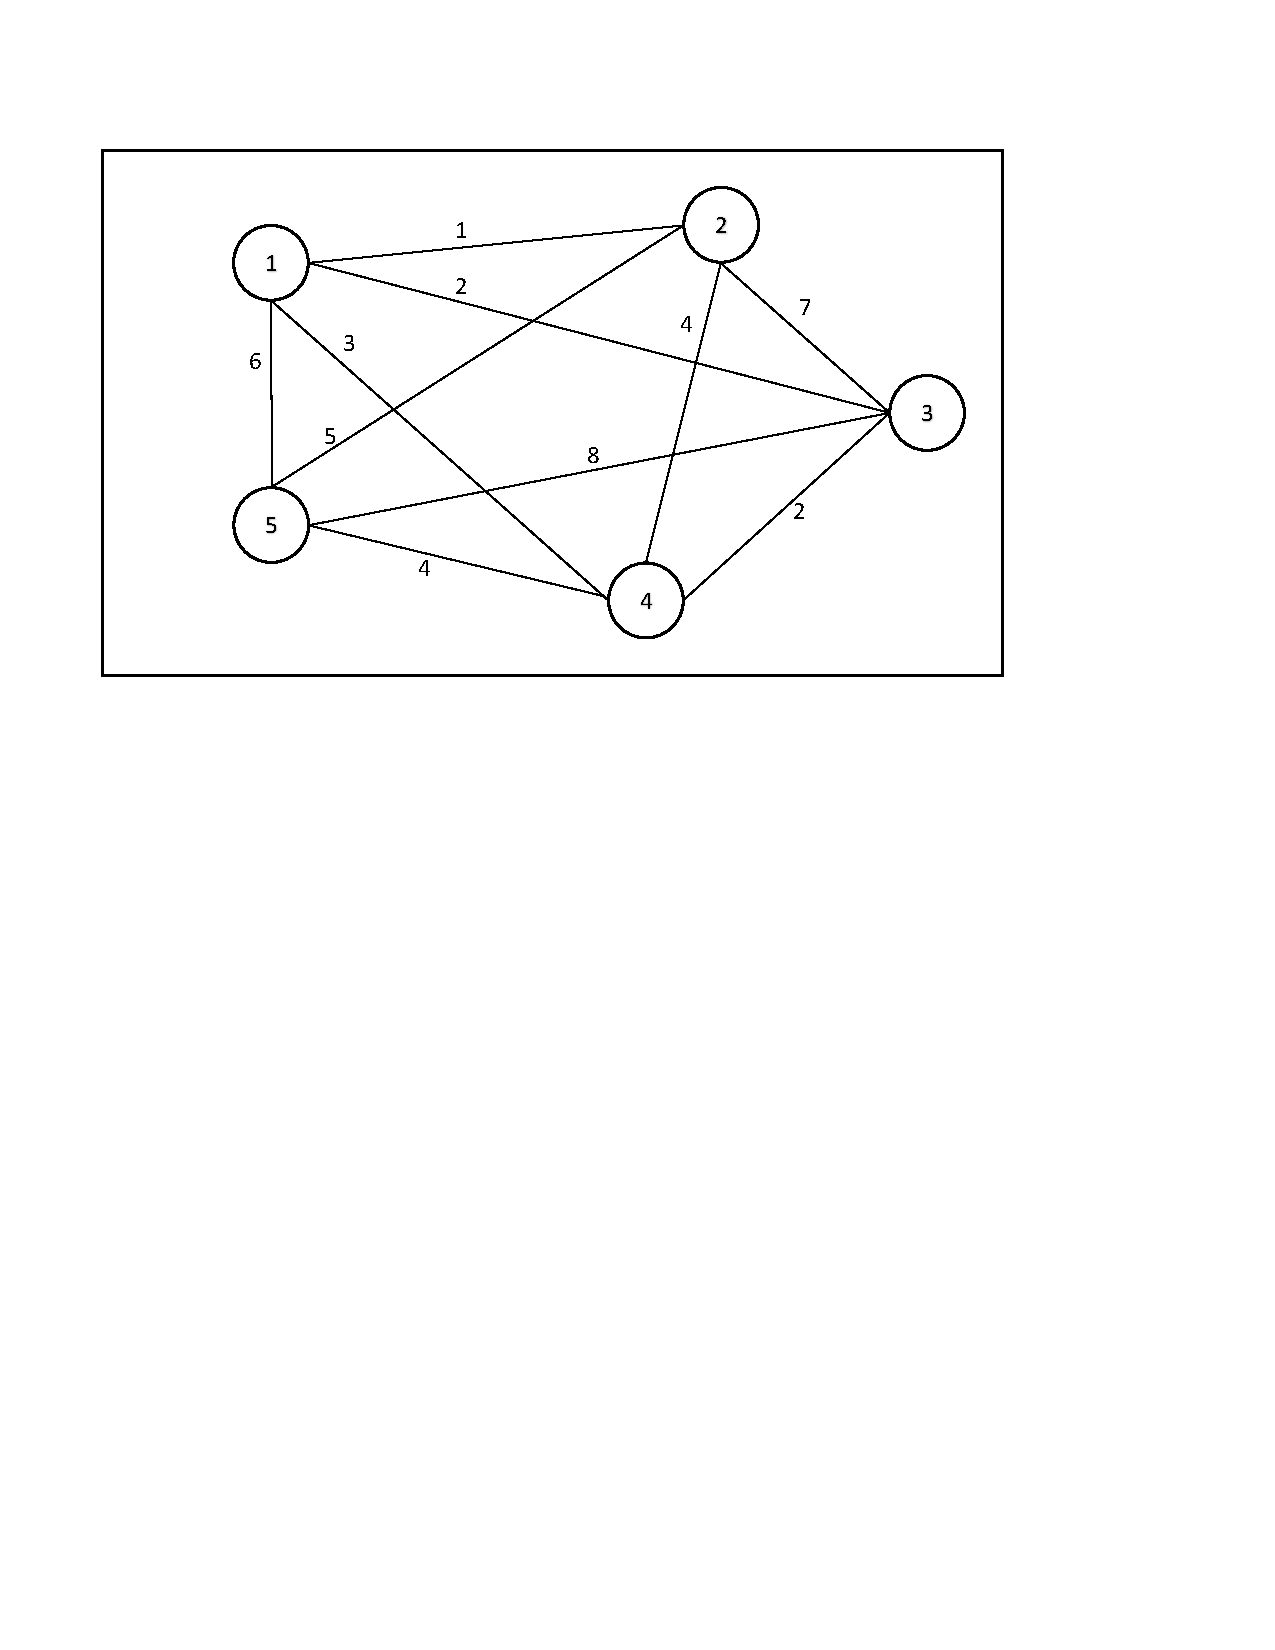
\includegraphics[width=.9\linewidth]{MetalSheetFig.pdf}
\end{multicols}


\begin{parts}
    
    \part[8] Formulate the metal manufacturer's task as an integer programming model in (abbreviated) \textbf{concrete} form. Clearly define all variables used and do NOT include subtour elimination constraints. \\
\answerboxone{c}{4.5in}

\newpage
	\part[2] For this particular problem, draw a solution that satisfies the constraints that you wrote, but is not a valid drill path OR explain why such a solution does not exist.

\answerboxone{c}{2in}

\vspace{.5cm}
    Reconsider the graph depicting the metal sheets.


\begin{center}
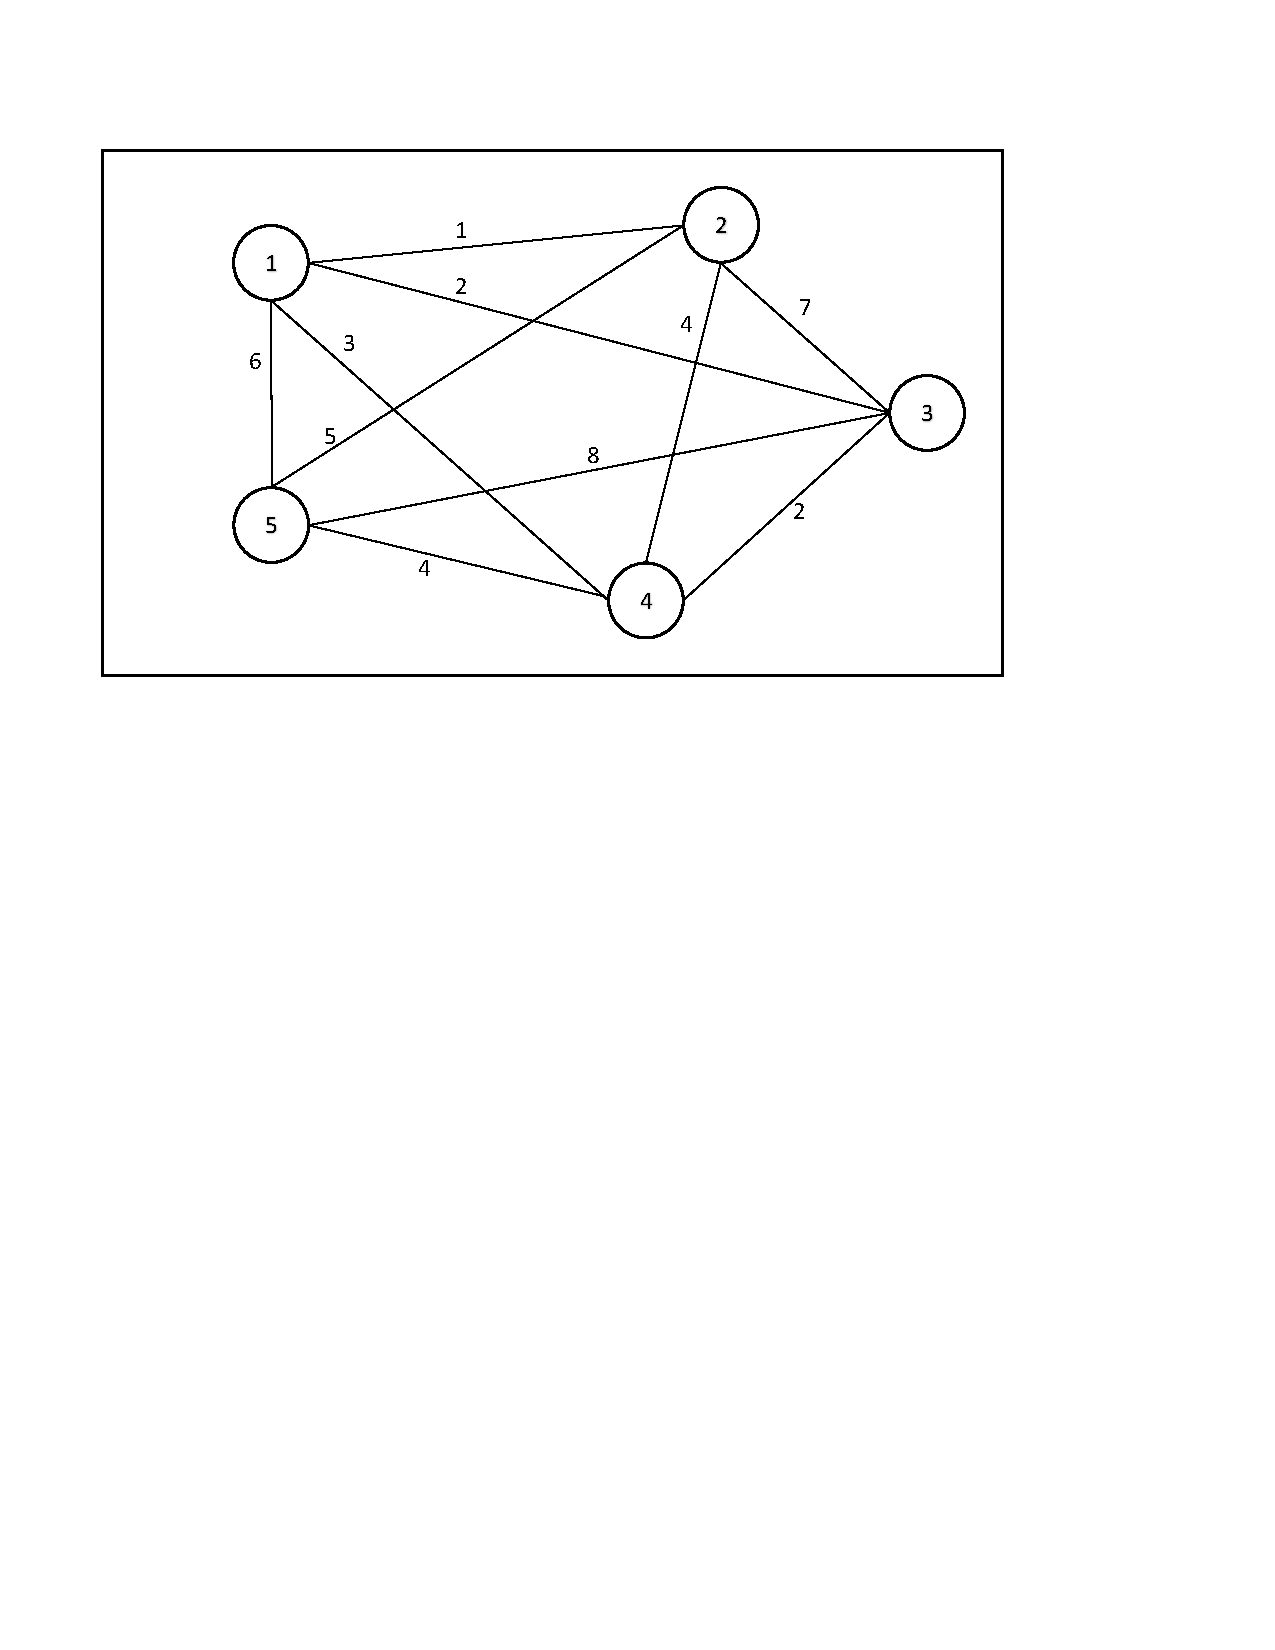
\includegraphics[width=.5\linewidth]{MetalSheetFig.pdf}
\end{center}


 
	\part[10] Run three iterations of the Nearest Neighbor method originating at holes 1, 3, and 5. Provide the respective sequences of nodes that begin at each of these nodes, along with the total time required for each sequence.\vspace{.5cm}
	
\answerboxone{c}{3in}
    
\end{parts}




\newpage
\question Your regional manager, Michael Scott, has asked you to solve a Vehicle Routing Problem (VRP) to determine an optimal set of 3 paper-delivery routes that begin and end at their warehouse in Scranton, PA. He also tells you that his goal is to minimize the total distance traveled among all vehicles.

\vspace{.5cm}
Answer the following questions related to Michael Scott's request.
\begin{parts}
\part[4] You solve the problem, and your solution contains a route of customers that does not contain the warehouse in Scranton. Does this solution provide an upper bound or a lower bound on your optimal vehicle routing solution? Justify your response.\\
\answerboxone{c}{1.7in}
\part[3] Now, Michael Scott tells you that each vehicle can travel no more than $D$ total miles on its route. Is this new problem a restriction or a relaxation of the original problem? Justify your response.\\
\answerboxone{c}{1.7in}
\part[3] Michael Scott also informs you that you are able, but not required, to use 4 vehicles instead of 3. Now, do you expect your optimal solution to this new problem to increase or decrease relative to the optimal solution to the original problem? Justify your response.\\
\answerboxone{c}{1.7in}
\end{parts}

\end{questions}



\end{document}


%\newpage
\question The Superintendent asks his most trusted Ops Research majors (you all) to give him directions from the Yard to Los Angeles, CA. Of course, he wants to find the path the minimizes his total travel time. Assume that he can travel through a set of cities $\mathcal{C}$ along a set of roads $\mathcal{A}$ between each city. He assumes that traveling along some arc $(i,j) \in \mathcal{A}$ will require $t_{ij} > 0$ minutes.  


\begin{parts}

\part Define your starting node $s$ and your destination/termination node $t$. Using these definitions, formulate an abstract mathematical programming model to help the superintendent solve his problem.

%\vspace{11cm}

\part The superintendent now wants to consider traffic delays in each city. To account for this added time it takes to travel through each city, he assumes that it will take $d_i > 0$ extra units of time to travel through city $i \in \mathcal{C}$. Modify your mathematical programming model above to account for the extra traffic-related time delays.
\end{parts}



\question[1] Calculate 2+2.
\addpoints

\question[20] Consider the function $f(x)=3x^3+2x^2+x+1$.
\noaddpoints % to omit double points count
\begin{parts}
\part[10] Calculate $f'(x)$.
\part[10] Calculate $f''(x)$.
\end{parts}
\addpoints

\question[2] One of these things is not like the others; one of these
things is not the same. Which one is different?
\begin{choices}
\choice John
\choice Paul
\choice George
\choice Ringo
\choice Socrates
\end{choices}

\question[2] One of these things is not like the others; one of these
things is not the same. Which one is different?
\begin{oneparchoices}
\choice John
\choice Paul
\choice George
\choice Ringo
\choice Socrates
\end{oneparchoices}

\question[3] Mark box if true.
\addpoints
\begin{checkboxes}
\choice 2+2=4
\choice $\frac{d}{dx} (x^2+1) = 2x+1$
\choice The Moon is made of cheese.
\end{checkboxes}

{%
\checkboxchar{$\Box$} % changing checkbox style locally
\question[3] Mark box if true.
\addpoints
\begin{checkboxes}
\choice 2+2=4
\choice $\frac{d}{dx} (x^2+1) = 2x+1$
\choice The Moon is made of cheese.
\end{checkboxes}
}%

{%
% changing choice items style locally
\renewcommand*\thechoice{\arabic{choice}} 
\renewcommand*\choicelabel{\thechoice)}
%
\question[2] Element with $Z=92$ is:
\begin{multicols}{2}
\begin{choices}
\choice H
\choice O
\choice F
\choice S
\choice Ba
\choice Pb
\choice U
\choice Pu
\end{choices}
\end{multicols}
}%

\question[10]
In no more than one paragraph, explain why the earth is round.
\makeemptybox{2in}

\question[20]
Explain blah, blah\ldots
\makeemptybox{\fill}

\newpage

\question[20]
Explain blah, blah\ldots
\fillwithlines{\fill}

\newpage

\question[20]
Explain blah, blah\ldots
\fillwithdottedlines{8em}







\end{questions}

\end{document}
